\chapter{Methods}
In this chapter, the methods used in this research are explained. First, the Coulomb Dissociation as a method for investigating the soft E1 excitation of neutron halo nuclei is described. For the Coulomb Dissociation, the concept of the reduced transition probability and the virtual photon method are introduced.
Secondly, the Invariant mass method utilized in the reconstruction of experimental data is explained, as well as the Equivalent photon method necessary for the extraction of the E1 reduced transition probability. 
Additionally, the Scattering angle method used for the study of dineutron correlation is also discussed.

\section{Coulomb Dissociation}
\begin{figure}[h]
    \centering
    \setlength{\unitlength}{1mm}
    \begin{picture}(100,30)
        % Boron-17 nucleus
        \put(10,20){\circle{15}}
        \put(10,22){\circle{10}}
        \put(7,21){\footnotesize ${}^{15}$B}
        \put(8,15){\circle*{2}}
        \put(12,15){\circle*{2}}
        \put(8,10){\footnotesize n     n}
        \put(6,29){${}^{17}$B}

        % Arrow to excited state
        \put(20,20){\vector(1,0){20}}

        % Excited Boron-17 nucleus
        \put(50,20){\circle{15}}
        \put(50,22){\circle{10}}
        \put(47,21){\footnotesize ${}^{15}$B}
        \put(48,15){\circle*{2}}
        \put(52,15){\circle*{2}}
        \put(48,10){\footnotesize n      n}
        %\put(50,20){\line(0,-1){12}}
        \put(50,3){\circle{12}}
        \put(48,4){\footnotesize Pb}
        \put(46,29){${}^{17}$B*}

        % Gamma ray
        \put(45,10){\line(-1,-2){5}}
        \put(37,3){\footnotesize $\gamma$}

        % Arrow to final state
        %\put(60,20){\vector(1,0){20}}

        % Final state boron-15
        \put(90,27){\circle{10}}
        \put(87,17){\footnotesize 15B}
        \put(60,20){\vector(1,0.3){20}}
        \put(92,29){\footnotesize \( E_{15B}, P_{15B} \)}

        % Final state neutron 1
        \put(90,13){\circle*{2}}
        \put(60,20){\vector(1,-0.3){20}}
        \put(92,13){\footnotesize \( E_{n1}, P_{n1} \)}
        % Final state neutron 2
        \put(90,10){\circle*{2}}
        \put(60,20){\vector(1,-0.5){20}}
        \put(92,10){\footnotesize \( E_{n2}, P_{n2} \)}

    \end{picture}
    \caption[Scheme of Coulomb Dissociation]{The scheme of Coulomb Dissociation of ${}^{17}$B. The ${}^{17}$B is induced to Pb target and excited by virtual photon made from electric magnetic field by ${}^{17}$B and Pb target. The excited ${}^{17}$B is dissociated into ${}^{15}$B and two neutrons. The $E$ and $\vec{P}$ are represent total energy and momentum of fragment respectively.}
\end{figure}

When nuclei is excited by the external electric field and breakup reaction occurs, the cross section of this reaction (Coulomb dissociation) can be written as follos,
\begin{align}
    \sigma_{CD} = \int N_{\gamma} (E_\gamma) \sigma_\gamma () dE_x,
\end{align}
Under the equivalent photon method\cite{Burtulani}, the coulomb dissociation cross section $(d\sigma(E1)/dE_x)$ can directly be described as,
\begin{align}
    \frac{d\sigma(E1)}{dE_x} = \frac{16 \pi^3}{9 \hbar c} N_{E1}(E_x) \frac{dB(E1)}{dE_x},
\end{align}
where $E_x$ is the excitation energy of nuclei, $N_{E1}(E_x)$ is the virtual photon number produced by E1 transition and $dB(E1) / dE_x$ is the E1 reduced transition probability. 



The virtual photon number for E1 transition is shown in Figure 2.2. The virtual photon number is obtained by investigating the photon flux at an impact parameter $b$ as,
\begin{align}
    N_{E1}(E_x) &= \int_{R}^{\infty} 2\pi b N_{E1}(E_x, b) db \notag \\
                &=\frac{2}{\pi}Z^{2}_{1}\alpha\Big(\frac{c}{v}\Big)^{2}\Big[\xi K_{0}(\xi)K_{1}(\xi)-\frac{v^{2}\xi^{2}}{2c^{2}}(K^{2}_{1}(\xi)-K^{2}_{0}(\xi)\Big]
\end{align}
where $\xi = E_x R / \gamma v \hbar$, $K_0, K_1$ are Modified Bessel function of order zero and one each,


The non-energy weighted sum rule of E1 transition is
\begin{align}
    B(E1) &= \int_{-\infty}^{\infty} \frac{dB(E1)}{dE_x}dE_x \notag \\
        &= \frac{3}{\pi} \bigg(\frac{Z e}{A}\bigg)^2 \langle r^2_{c-nn} \rangle \notag \\
        &= \frac{3}{4 \pi} \bigg(\frac{Z e}{A}\bigg)^2 \langle \vec{r_1}^2 + \vec{r_2}^2 + 2 \vec{r_1} \cdot \vec{r_2} \rangle \notag \\
        &= \frac{3}{4 \pi} \bigg(\frac{Z e}{A}\bigg)^2 \langle \vec{r_1}^2 + \vec{r_2}^2 + 2\vec{r_1} \vec{r_2} \cos \theta_{12} \rangle
\end{align}


\begin{figure}[t]
    \centering
    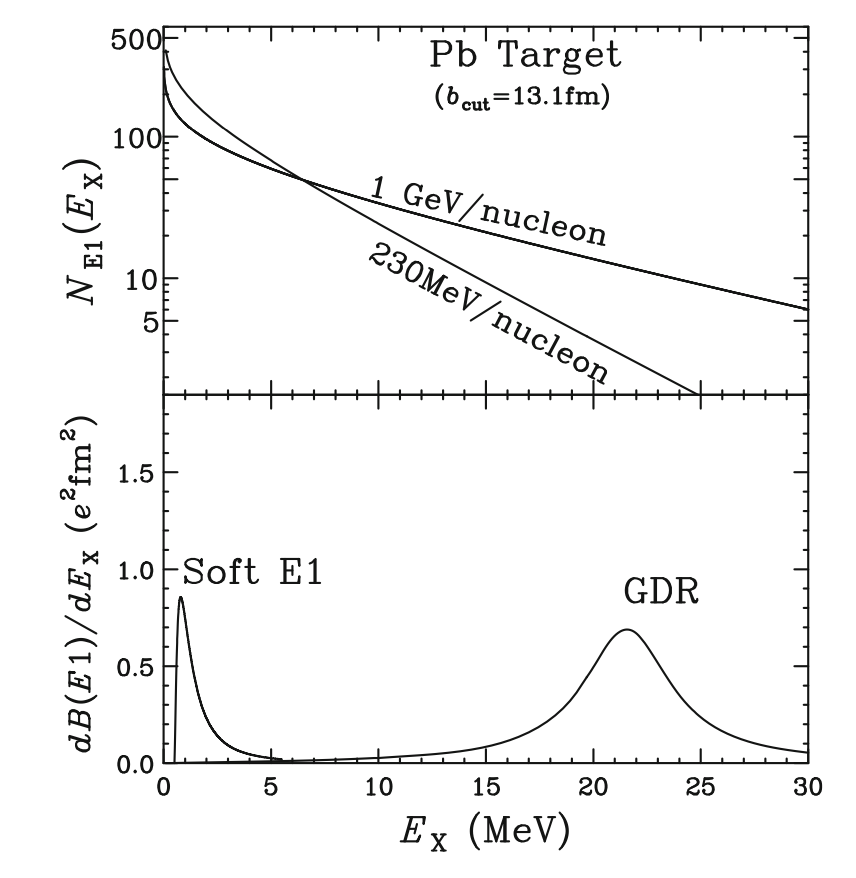
\includegraphics[width=8cm]{chapter2/Virtual_Photon.png}
    \caption[Virtual Photon Spectra and E1 Modes]{Virtual photon spectra and E1 modes.}
\end{figure}

\subsection{Cross Section Extraction}

\begin{align}
    \sigma_{CD} = \sigma(Pb) - \Gamma \sigma(C),
\end{align}
Where $\Gamma$ represent the ratio of the cross section 


\section{Invariant Mass Method}
To investigate the ${}^{17}$B, invariant mass method is used. The invariant mass method is a method to reconstruct the excited state of the system by measuring the momentum and energy of the fragments. The invariant mass of the system is defined as
\begin{align}
    M^* &= \sqrt{\bigg(\sum_{i} E_i\bigg)^2 - \bigg(\sum_{i}\vec{P}_i \bigg)^2} 
\end{align}

\begin{align}
    E_{rel} &= M({}^{17}\text{B}^*) - (m_{{}^{15}\text{B}} + 2m_n)
\end{align}
%Assuming two-body decay, the invariant mass of the system can be written as
%\begin{align}
%    E_{rel} &= \sqrt{(E_1 + E_2)^2 - (\vec{P}_1 + \vec{P}_2)^2} - m_1 - m_2\\
%    &= \sqrt{m_1^2 + m_2^2 + 2(E_1E_2 - |\vec{P}_1||\vec{P}_2|\text{cos} \theta_{12} )} - m_1 - m_2
%\end{align}

\section{Geometrical Correlation}
\begin{figure}[t]
    \centering
    \setlength{\unitlength}{1mm}
    \begin{picture}(60,40)
        \put(5,15){$E_x$}
        \put(16,1){${}^{17}$B}
        \put(18,31){$M$}
        %\put(10,0){\dashbox{dash-len}}}
        \thicklines
        \put(10,30){\line(1,0){20}}
        \put(10,0){\line(1,0){20}}
        \put(50,10){\line(1,0){20}}
        \put(20,5){\vector(0,1){24}}
        \put(31,29){\vector(1,-1){18}}
        \thinlines
        \multiput(34,10)(1.2,0){15}{\line(1,0){0.8}}
        \multiput(30,0)(1.2,0){10}{\line(1,0){0.8}}
    \end{picture}    
\end{figure}


\begin{align}
    \langle r^2_m \rangle = \frac{A_c}{A}\langle r^2_m \rangle_c + \frac{2A_c}{A^2}\langle r^2_{c-nn} \rangle + \frac{1}{2A}\langle r^2_{nn} \rangle
\end{align}


\begin{figure}[h]
    \centering
    \setlength{\unitlength}{1mm}
    \begin{picture}(100,30)
      % GDR
      \put(70,20){\circle{20}} % GDR
      \put(72,20){\circle{20}} % GDR
      \put(70,20){\vector(1,0){3}}%
      \put(70,20){\vector(-1,0){2}}%
      \put(63,30){$p$} % p label
      \put(77,30){$n$} % n label
      \put(67,5){GDR} % GDR label
    
      % Soft E1
      \put(20,20){\circle{18}}
      \put(23,20){\circle*{10}}
        \put(15,20){\vector(1,0){2}}
        \put(15,20){\vector(-1,0){2}}
        \put(15,5){Soft $E1$}
        
    \end{picture}
    \caption{The schematic representation of the giant dipole resonance and soft dipole mode}
    \end{figure}